\subsection{Wheelchair Fencing}

\begin{enumerate}

\item Essence of Wheelchair Fencing
    \begin{itemize}
    \item Wheelchair fencing is a strategic and elegant combat sport that showcases the precision, agility, and tactical acumen of athletes with physical impairments. 
    \item Seated in wheelchairs that are securely fastened to the piste (fencing strip), athletes engage in duels using épée, foil, or sabre weapons, aiming to touch their opponents with the tip of their blade. 
    \item The sport demands lightning-fast reflexes, precise movements, and strategic thinking, creating a captivating display of skill and athleticism.
    \end{itemize}

\item Rules, Equipment, and Competition
    \begin{itemize}
    \item Wheelchair fencing adheres to the fundamental rules of fencing, with adaptations for athletes with impairments. 
    \item The wheelchairs are fixed to the piste, and athletes use modified grips and techniques to wield their weapons. 
    \item The competition format involves individual and team events, with fencers competing in different categories based on their weapon and classification. 
    \item Matches are won by scoring the most touches within a set time or reaching a certain number of points first.
    \end{itemize}

\item Categories and Classifications
    \begin{itemize}
    \item Wheelchair fencing utilizes a classification system based on the athlete's trunk control and fencing arm mobility. 
    \item There are two main categories: 
        \begin{itemize}
        \item Category A for athletes with good trunk control and fencing arm mobility
        \item Category B for those with limited trunk control or impaired fencing arm function
        \end{itemize} 
    \item This classification ensures fair competition and allows athletes with different levels of impairment to showcase their fencing skills and compete against others with comparable abilities.
    \end{itemize}

\begin{figure}[htbp] % htbp are float placement options
\centering
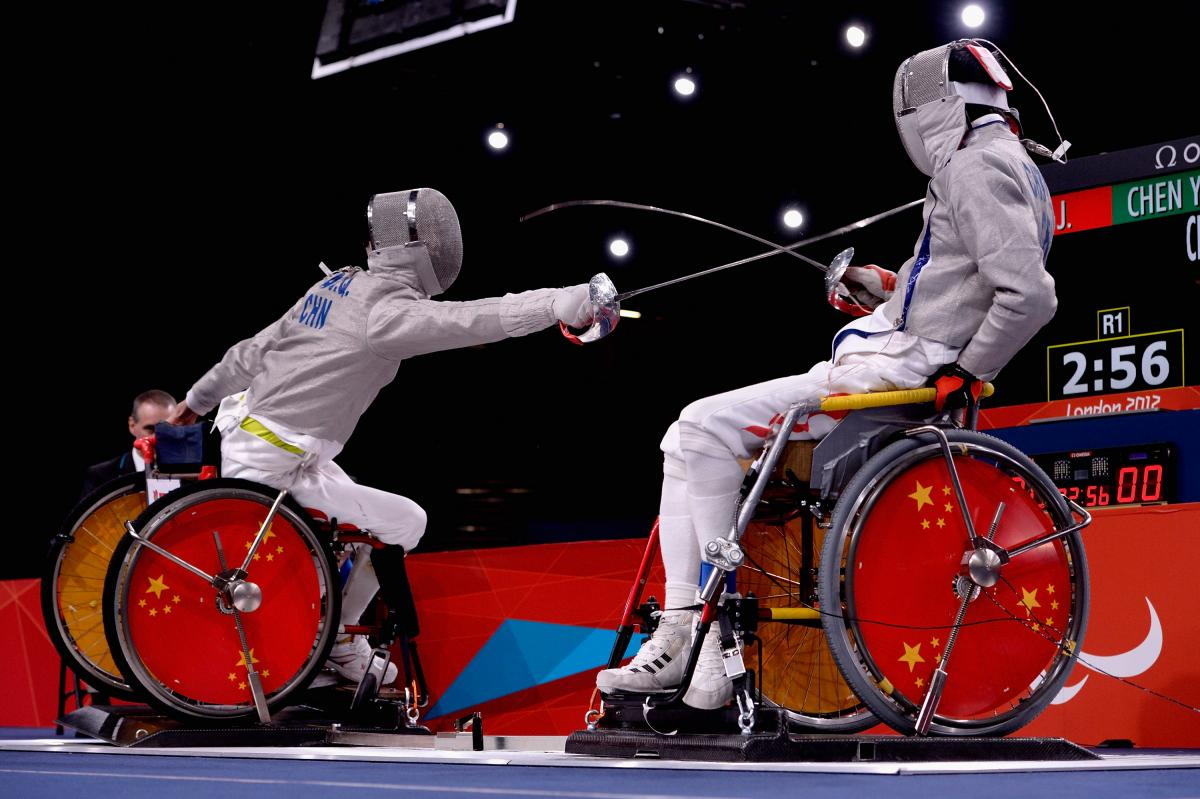
\includegraphics[width=0.8\textwidth]{Images/weelchair_fencing.jpg}
\caption{Weelchair fencing}
\label{fig:my_image}
\end{figure}

\end{enumerate}